\documentclass[11pt,border=5pt]{standalone}
\usepackage{amsmath,amssymb}
\usepackage{tikz}
\usetikzlibrary{arrows.meta,positioning,calc,shapes.misc,shapes.geometric,backgrounds}
\newcommand{\Aset}{\mathcal{A}}
\definecolor{cL1}{HTML}{C44E52}
\definecolor{cL2}{HTML}{DD8452}
\definecolor{cL3}{HTML}{8172B3}
\definecolor{cOK}{HTML}{55A868}
\definecolor{cIn}{HTML}{5B6B7F}
\definecolor{cDef}{HTML}{8C8C8C}
\definecolor{cBox}{HTML}{1F77B4}
\begin{document}
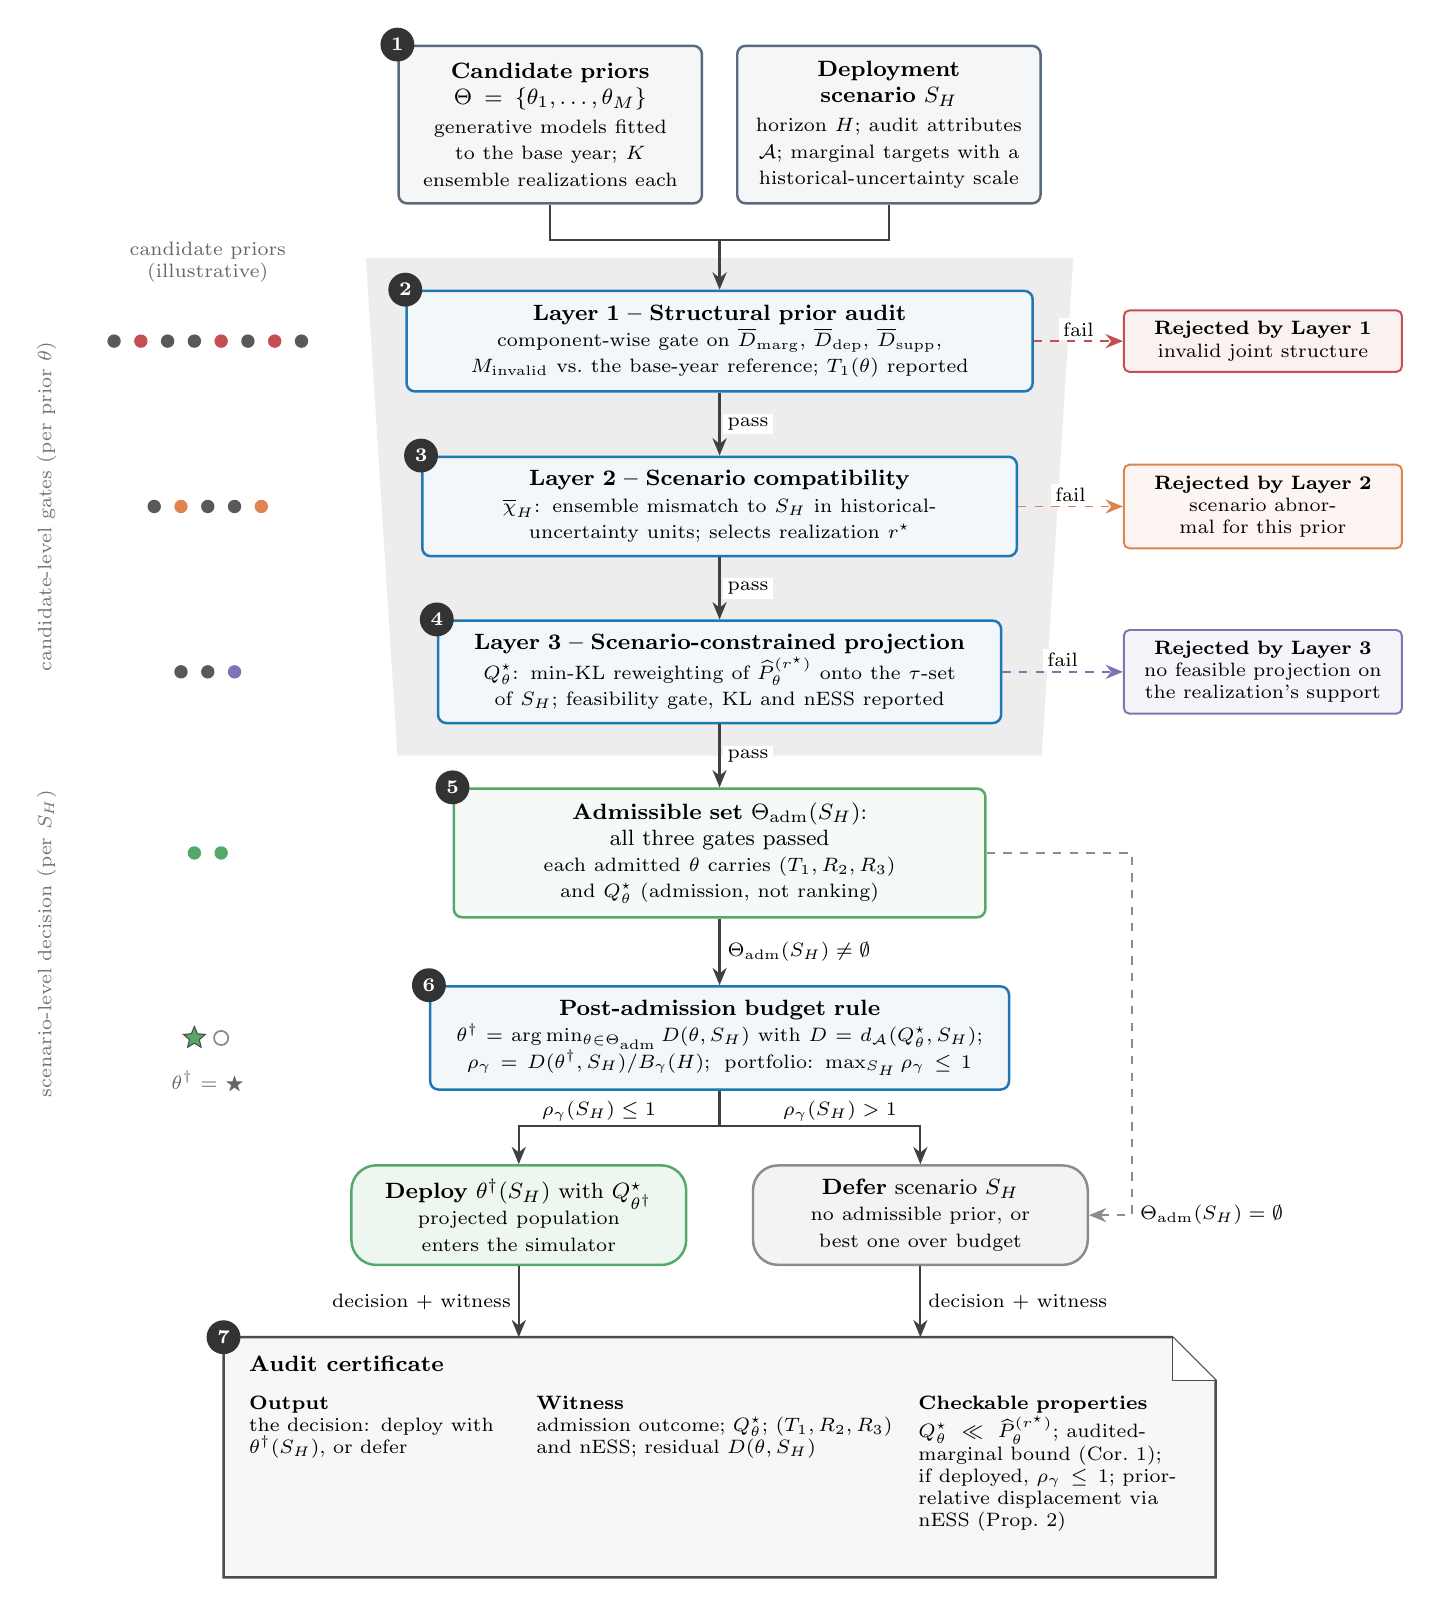
\begin{tikzpicture}[
  font=\footnotesize,
  >={Stealth[length=2.2mm,width=1.8mm]},
  flow/.style={->, line width=0.8pt, draw=black!75},
  fail/.style={->, line width=0.7pt, draw=#1, dashed},
  main/.style={draw=#1, line width=0.9pt, fill=#1!6, rounded corners=3pt, align=center, inner sep=5pt, text width=7.2cm},
  rej/.style={draw=#1, line width=0.7pt, fill=#1!8, rounded corners=2pt, align=center, inner sep=4pt, text width=3.25cm, font=\scriptsize},
  pill/.style={draw=#1, line width=0.9pt, fill=#1!10, rounded corners=9pt, align=center, inner sep=5pt, text width=3.9cm},
  stepno/.style={circle, fill=black!80, text=white, font=\scriptsize\bfseries, inner sep=1pt, minimum size=4.3mm},
  lab/.style={font=\scriptsize, fill=white, inner sep=1.5pt},
  dot/k/.style={circle, fill=black!65, inner sep=0pt, minimum size=1.7mm},
  dot/g/.style={circle, fill=cOK, inner sep=0pt, minimum size=1.7mm},
  dot/h/.style={circle, draw=black!47, line width=0.6pt, fill=white, inner sep=0pt, minimum size=1.8mm},
  dot/r1/.style={circle, fill=cL1, inner sep=0pt, minimum size=1.7mm},
  dot/r2/.style={circle, fill=cL2, inner sep=0pt, minimum size=1.7mm},
  dot/r3/.style={circle, fill=cL3, inner sep=0pt, minimum size=1.7mm},
  dot/s/.style={star, star points=5, star point ratio=2.2, fill=cOK, draw=black!70, line width=0.4pt, inner sep=0pt, minimum size=2.9mm},
]
% ================= step 1: inputs =================
\node[main=cIn, text width=3.5cm, minimum height=2.0cm] (in1) at (-2.15,0)
 {\textbf{Candidate priors}\\ $\Theta=\{\theta_1,\ldots,\theta_M\}$\\[1pt]
  {\scriptsize generative models fitted to the base year; $K$ ensemble realizations each}};
\node[main=cIn, text width=3.5cm, minimum height=2.0cm] (in2) at (2.15,0)
 {\textbf{Deployment scenario} $S_H$\\[1pt]
  {\scriptsize horizon $H$; audit attributes $\Aset$; marginal targets with a historical-uncertainty scale}};
% ================= steps 2-4: layers =================
\node[main=cBox, text width=7.6cm] (L1) at (0,-2.75)
 {\textbf{Layer 1 -- Structural prior audit}\\
  {\scriptsize component-wise gate on $\overline D_{\mathrm{marg}}$, $\overline D_{\mathrm{dep}}$, $\overline D_{\mathrm{supp}}$, $M_{\mathrm{invalid}}$ vs.\ the base-year reference; $T_1(\theta)$ reported}};
\node[main=cBox, text width=7.2cm] (L2) at (0,-4.85)
 {\textbf{Layer 2 -- Scenario compatibility}\\
  {\scriptsize $\overline{\chi}_H$: ensemble mismatch to $S_H$ in historical-uncertainty units; selects realization $r^\star$}};
\node[main=cBox, text width=6.8cm] (L3) at (0,-6.95)
 {\textbf{Layer 3 -- Scenario-constrained projection}\\
  {\scriptsize $Q^\star_\theta$: min-KL reweighting of $\widehat P^{(r^\star)}_\theta$ onto the $\tau$-set of $S_H$; feasibility gate, KL and $\mathrm{nESS}$ reported}};
% ================= step 5: admissible set =================
\node[main=cOK, text width=6.4cm] (adm) at (0,-9.25)
 {\textbf{Admissible set} $\Theta_{\mathrm{adm}}(S_H)$: all three gates passed\\
  {\scriptsize each admitted $\theta$ carries $(T_1,R_2,R_3)$ and $Q^\star_\theta$ (admission, not ranking)}};
% ================= step 6: budget rule =================
\node[main=cBox, text width=7.0cm] (bud) at (0,-11.6)
 {\textbf{Post-admission budget rule}\\
  {\scriptsize $\theta^\dagger=\arg\min_{\theta\in\Theta_{\mathrm{adm}}}D(\theta,S_H)$ with $D=d_{\Aset}(Q^\star_\theta,S_H)$;\;
   $\rho_\gamma=D(\theta^\dagger,S_H)/B_\gamma(H)$;\; portfolio: $\max_{S_H}\rho_\gamma\le 1$}};
\node[pill=cOK] (dep) at (-2.55,-13.85)
 {\textbf{Deploy} $\theta^\dagger(S_H)$ with $Q^\star_{\theta^\dagger}$\\ {\scriptsize projected population enters the simulator}};
\node[pill=cDef] (def) at (2.55,-13.85)
 {\textbf{Defer} scenario $S_H$\\ {\scriptsize no admissible prior, or best one over budget}};
% ================= step 7: certificate (document shape) =================
\coordinate (cNW) at (-6.3,-15.4);
\coordinate (cSE) at (6.3,-18.45);
\path[draw=black!70, fill=black!3, line width=0.9pt]
  (cNW) -- ($(cSE |- cNW)+(-0.55,0)$) -- ($(cSE |- cNW)+(0,-0.55)$) -- (cSE) -- (cNW |- cSE) -- cycle;
\path[draw=black!70, fill=white, line width=0.6pt]
  ($(cSE |- cNW)+(-0.55,0)$) -- ($(cSE |- cNW)+(-0.55,-0.55)$) -- ($(cSE |- cNW)+(0,-0.55)$);
\node[anchor=north west, font=\footnotesize\bfseries] at ($(cNW)+(0.2,-0.12)$) {Audit certificate};
\node[anchor=north west, align=left, text width=3.3cm, font=\scriptsize] at ($(cNW)+(0.2,-0.62)$)
 {\textbf{Output}\\ the decision: deploy with $\theta^\dagger(S_H)$, or defer};
\node[anchor=north west, align=left, text width=4.6cm, font=\scriptsize] at ($(cNW)+(3.85,-0.62)$)
 {\textbf{Witness}\\ admission outcome; $Q^\star_\theta$; $(T_1,R_2,R_3)$ and $\mathrm{nESS}$; residual $D(\theta,S_H)$};
\node[anchor=north west, align=left, text width=3.6cm, font=\scriptsize] at ($(cNW)+(8.7,-0.62)$)
 {\textbf{Checkable properties}\\ $Q^\star_\theta\ll\widehat P^{(r^\star)}_\theta$; audited-marginal bound (Cor.~1); if deployed, $\rho_\gamma\le 1$; prior-relative displacement via nESS (Prop.~2)};
% ================= reject bins =================
\node[rej=cL1] (r1) at (6.9,-2.75)
 {\textbf{Rejected by Layer 1}\\ invalid joint structure};
\node[rej=cL2] (r2) at (6.9,-4.85)
 {\textbf{Rejected by Layer 2}\\ scenario abnormal for this prior};
\node[rej=cL3] (r3) at (6.9,-6.95)
 {\textbf{Rejected by Layer 3}\\ no feasible projection on the realization's support};
% ================= funnel background =================
\begin{scope}[on background layer]
\fill[black!7] ($(L1.north west)+(-0.5,0.4)$) -- ($(L1.north east)+(0.5,0.4)$)
             -- ($(L3.south east)+(0.5,-0.4)$) -- ($(L3.south west)+(-0.5,-0.4)$) -- cycle;
\end{scope}
% ================= arrows =================
\coordinate (j) at ($(L1.north |- in1.south)+(0,-0.45)$);
\draw[line width=0.8pt, draw=black!75] (in1.south) -- (in1.south |- j) -- (in2.south |- j) -- (in2.south);
\draw[flow] (j) -- (L1.north);
\draw[flow] (L1) -- node[lab, right=1pt] {pass} (L2);
\draw[flow] (L2) -- node[lab, right=1pt] {pass} (L3);
\draw[flow] (L3) -- node[lab, right=1pt] {pass} (adm);
\draw[fail=cL1] (L1.east) -- node[lab, above] {fail} (r1.west);
\draw[fail=cL2] (L2.east) -- node[lab, above] {fail} (r2.west);
\draw[fail=cL3] (L3.east) -- node[lab, above] {fail} (r3.west);
\draw[flow] (adm) -- node[lab, right=1pt] {$\Theta_{\mathrm{adm}}(S_H)\neq\emptyset$} (bud);
\draw[fail=cDef] (adm.east) -| ($(def.east)+(0.55,0)$) -- node[lab, pos=0.5, right=1pt] {$\Theta_{\mathrm{adm}}(S_H)=\emptyset$} ($(def.east)+(0.55,0)$) -- (def.east);
\draw[flow] (bud.south) -- ++(0,-0.45) -| node[lab, pos=0.3, above] {$\rho_\gamma(S_H)\le 1$} (dep.north);
\draw[flow] (bud.south) -- ++(0,-0.45) -| node[lab, pos=0.3, above] {$\rho_\gamma(S_H)> 1$} (def.north);
\draw[flow] (dep.south) -- node[lab, left=1pt] {decision + witness} (dep.south |- cNW);
\draw[flow] (def.south) -- node[lab, right=1pt] {decision + witness} (def.south |- cNW);
% ================= step badges =================
\node[stepno] at (in1.north west) {1};
\node[stepno] at (L1.north west) {2};
\node[stepno] at (L2.north west) {3};
\node[stepno] at (L3.north west) {4};
\node[stepno] at (adm.north west) {5};
\node[stepno] at (bud.north west) {6};
\node[stepno] at (cNW) {7};
% ================= candidate strips (illustrative) =================
\node[font=\scriptsize, align=center, text=black!60] at (-6.5,-1.75) {candidate priors\\ (illustrative)};
\foreach \y/\n/\lst in {-2.75/8/{k,r1,k,k,r1,k,r1,k}, -4.85/5/{k,r2,k,k,r2}, -6.95/3/{k,k,r3}, -9.25/2/{g,g}, -11.6/2/{s,h}}
 {\foreach [count=\i] \s in \lst {\node[dot/\s] at ({-6.5+0.34*(\i-(\n+1)/2)},\y) {};}}
\node[font=\scriptsize, text=black!60, anchor=north] at (-6.5,-11.9) {$\theta^\dagger$ = $\bigstar$};
% ================= side labels =================
\node[rotate=90, font=\scriptsize, text=black!55, anchor=south] at (-8.3,-4.85) {candidate-level gates (per prior $\theta$)};
\node[rotate=90, font=\scriptsize, text=black!55, anchor=south] at (-8.3,-10.4) {scenario-level decision (per $S_H$)};
\end{tikzpicture}
\end{document}
